\newpage
\section{Consuntivo di periodo}

In base ai consuntivi di periodo dei periodi completati sono state effettuate le diverse modifiche alla pianificazione per rientrare nel budget preventivato al momento della consegna per aggiudicarci il capitolato.
Di seguito sarà descritto il consuntivo di periodo di \VV.

\subsection{\VV}
La differenza di costi tra quelli preventivati nella sezione 5 di questo documento e quello effettivamente speso è la seguente:

\begin{table}[h]
	\begin{center}
		\begin{tabular}{|c|c|c|c|c|c|}
			\hline
			\textbf{Ruolo}	& \textbf{Ore Preventivate} & \textbf{Costo preventivato} &  \textbf{Differenza ore} & \textbf{Differenza costo} \\
			\hline
			\Pm &	8 & 240 & 0 & 0\\
			\hline
			\Am	&	3 & 60 & +2 & +40\\
			\hline
			\Prog	&	6 & 132 & -1 & -22\\
			\hline
			\Progr	&	8 & 120 & -2 & -30\\
			\hline
			\Ver	&	53 & 795 & +2 & +30\\
			\hline
			\textbf{totale}	&	\textbf{78} & \textbf{1347} & \textbf{+1} & \textbf{+18}\\
			\hline
		\end{tabular}
	\end{center}
	\caption{Consuntivo di periodo \VV}
\end{table}

\begin{figure}[H]
	\centering
	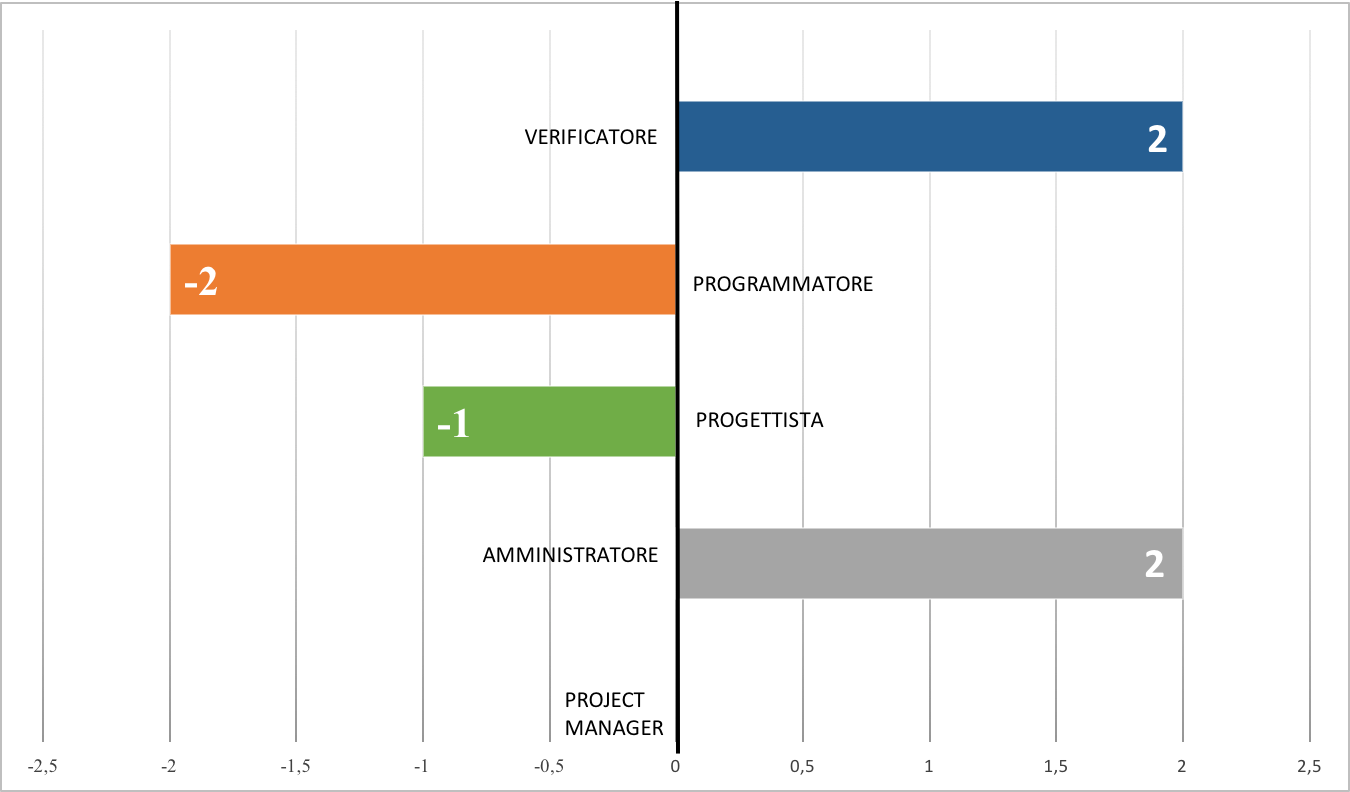
\includegraphics[scale=0.7]{Immagini/GraficiCONS/DIFFCONSP.png}
	\caption{Differenza oraria per ruolo a consuntivo, Consuntivo di periodo \VV}
\end{figure}

\newpage

\section{Consuntivo}
Di seguito sarà descritto il consuntivo di progetto.\\
La tabella seguente illustra le ore totali a consuntivo che ogni componente ha dedicato per il progetto, mettendo in evidenza anche quelle rendicontate. Le ore non rendicontate corrispondono alle ore dedicate al primo periodo (\ARM) che, come già esplicato in precedenza, rappresenta l'investimento iniziale del \termine{gruppo} per aggiudicarsi il capitolato e comprendono, oltre ad attività di auto-apprendimento, tutte le attività svolte nel periodo di \ARM\ (§3.2.1). Inoltre, come descritto in nella sezione 4, sono state previste ulteriori ore di autoapprendimento (durante il periodo di \PD\ e \COD\ da \RP\ fino a \RQ) in seguito al verificarsi del rischio tecnologico relativo alla difficile comprensione di alcune tecnologie, in particolare la difficile comprensione della documentazione della piattaforma \termine{Rocket.chat}.

\begin{table}[h]
	\begin{center}
		\begin{tabular}{|c|c|c|c|c|c|c|c|c|}
			\hline
			\multirow{2}{*} {\textbf{Nominativo}} & & \multicolumn{6}{c|}{\textbf{Ore per ruolo}} & \multirow{2}{*}{\textbf{Ore totali}} \\
			& & PM & AM & AN & PT & PR & VE & \\
			\hline
			\multirow{2}{*}{\FB}		&	Rendicontate	&	8	&	0	&	6	&	41 & 24	&	26 & 105	\\
			\cline{2-9}
			&	Totali			&	8	& 4	&	16	&	41	&	32	& 40 &	141	\\
			\hline
			\multirow{2}{*}{\RM}	&	Rendicontate	&	4 &	3	&	6	&	32	&	16	&  44	&	105	\\
			\cline{2-9}
			&	Totali			&	9	&	3	&	12	&	32	&	24	& 	61	&	141	\\
			\hline
			\multirow{2}{*}{\SL}	&	Rendicontate	&	4	&	8	&	0	&	36	&	23	&	34	&	105	\\	
			\cline{2-9}
			&	Totali			&	12	&	14	&	11	&	36	&	31	& 36 	&	140	\\
			\hline
			\multirow{2}{*}{\DC}	&	Rendicontate	&	3	&	5	&	7	&	42	&	14	&	34	&	105	\\	
			\cline{2-9}
			&	Totali			&	3	&	6	&	15	&	42	&	22	&	53	&	141	\\
			\hline
			\multirow{2}{*}{\LD}		&	Rendicontate	&	3	&	0	&	6	& 18 	&	30	& 	48	&	105	\\	
			\cline{2-9}
			&	Totali			&	10	&	2	&	15	&	18	&	38	& 	57	&	140	\\
			\hline
			\multirow{2}{*}{\MT}	&	Rendicontate	&	5	&	5	&	5	&	25	&	23	& 	42	&	105	\\
			\cline{2-9}
			&	Totali			&	5	&	5	&	17	&	25	&	31	& 	58	&	140	\\
			\hline
			\multirow{2}{*}{\ND}	&	Rendicontate	&	10	&	6	&	0	&	38	&	20	& 	31	&	105	\\	
			\cline{2-9}
			&	Totali	&	10	&	12	&	19	&	38	&	28	& 	33	&	140	\\
			\hline
		\end{tabular}
	\end{center}
	\caption{Ore per componente per ruolo a consuntivo, rendicontate e totali}
\end{table}

\begin{figure}[H]
	\centering 
	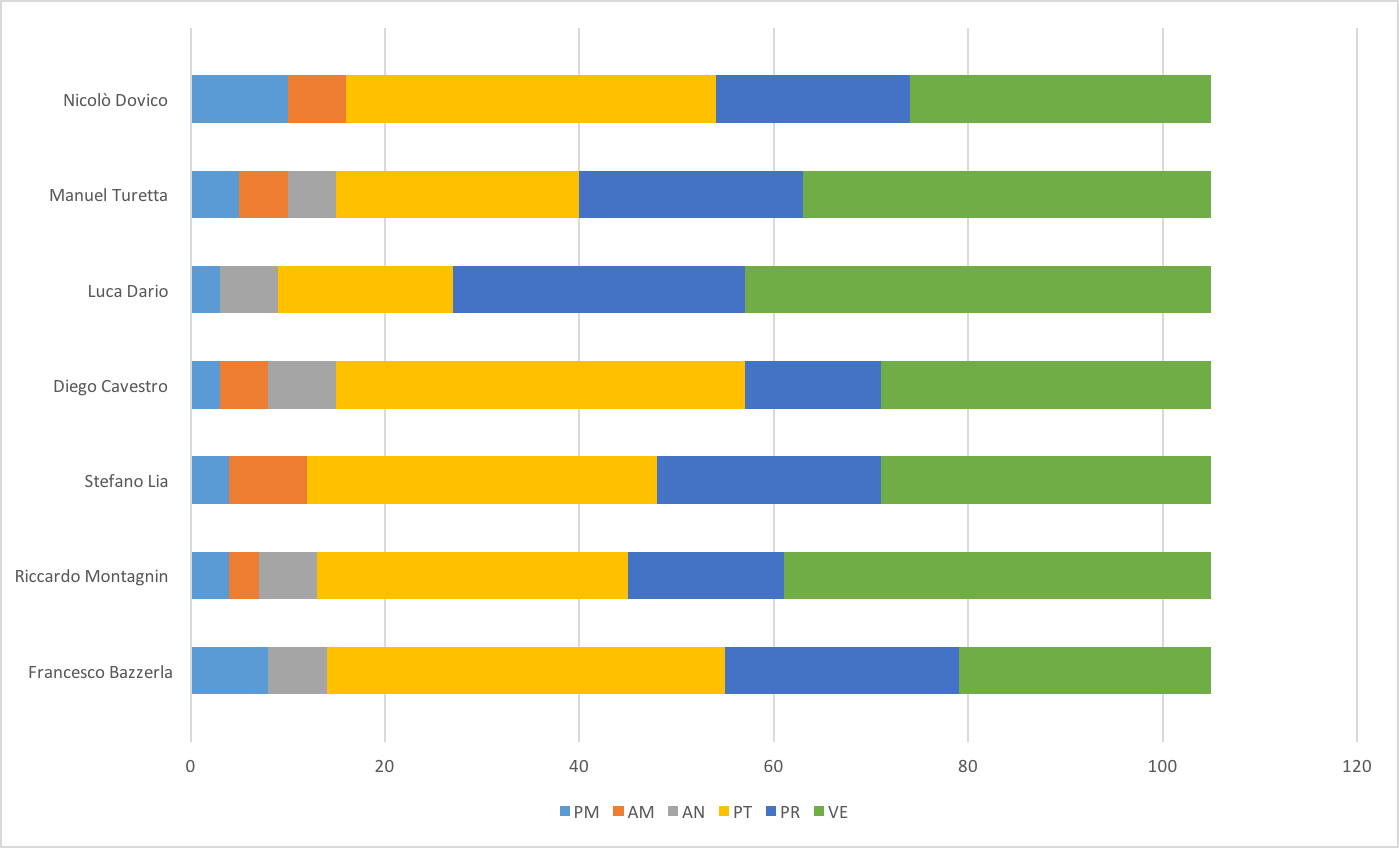
\includegraphics[scale=0.6]{Immagini/GraficiCONS/DIVLAVCONS.png}
	\caption{Incidenza ore rendicontate per membro a consuntivo}
\end{figure}

In particolare la differenza di costi totali tra quelli preventivati nella sezione 5 di questo documento e quello effettivamente speso è la seguente:

\begin{table}[h]
	\begin{center}
		\resizebox{\textwidth}{!}{\begin{tabular}{|l|c|c|c|c|c|c|}
			\hline
			\textbf{Ruolo}	& \textbf{Ore preventivate} & \textbf{Ore finali} &	\textbf{Ore remunerabili preventivate} &	\textbf{Ore remunerabili finali}	 &\textbf{Costo preventivato} & \textbf{Costo finale}  \\
			\hline
			\textit{\Pm}	&	57 & 57	&	37 & 37	&	1110 & 1110	\\
			\hline
			\textit{\Am}	&	44 & 46	&	25 & 27	&	500 & 540	\\
			\hline
			\textit{\An}	&	105 & 105	&	30 & 30	&	750 & 750	\\
			\hline
			\textit{\Prog}	&	233 & 232	&	233 & 232	&	5126 & 5104	\\
			\hline
			\textit{\Progr}	&	208 & 207	&	152 & 150	&	2280 & 2250	\\
			\hline
			\textit{\Ver}	&	336 & 338	&	257 & 259	&	3855 & 3885	\\
			\hline
			\textbf{Totale}	&	\textbf{983} &	\textbf{984} & \textbf{734} & \textbf{735} & \textbf{13621} & \textbf{13639}	\\
			\hline
		\end{tabular}
		}
	\end{center}
	\caption{Costo totale per ruolo a consuntivo}
\end{table}

\begin{figure}[H]
	\centering 
	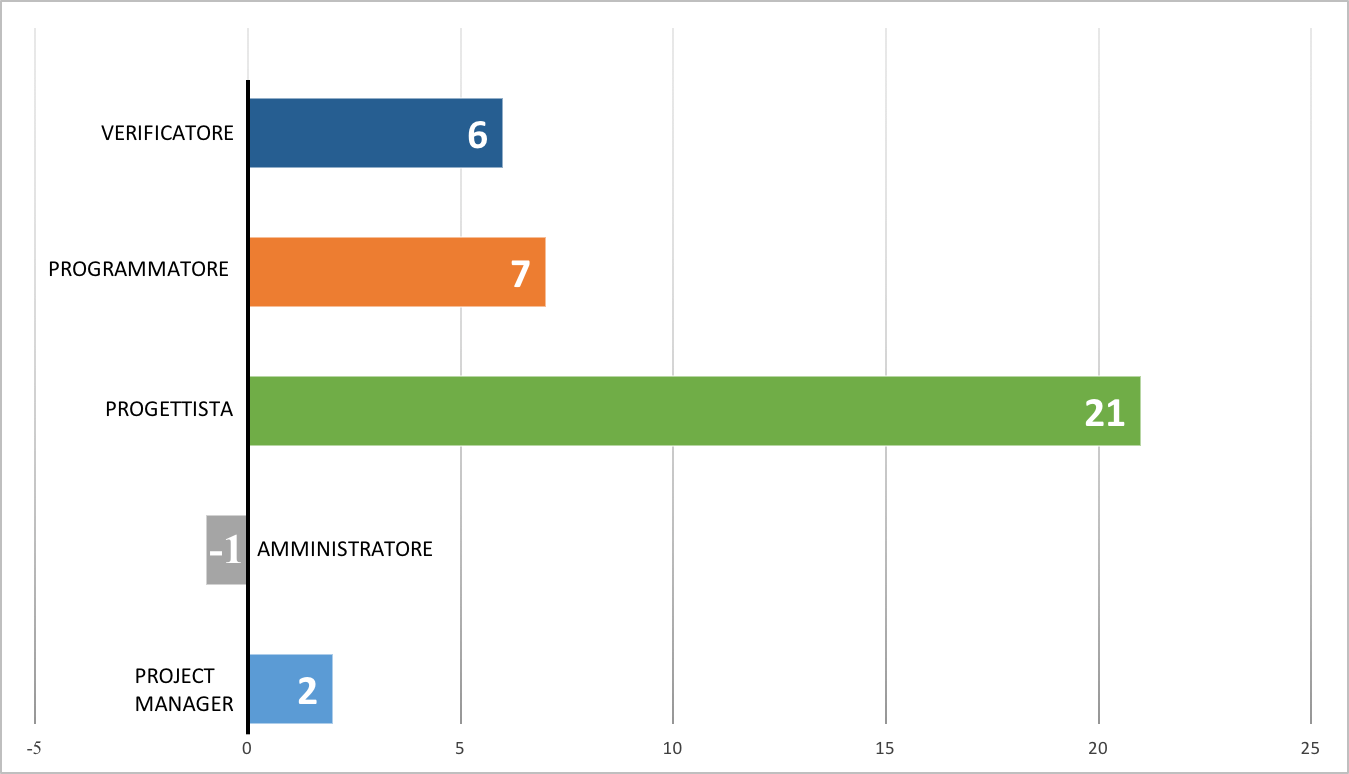
\includegraphics[scale=0.7]{Immagini/GraficiCONS/DIFFCONS.png}
	\caption{Costo totale per ruolo a consuntivo}
\end{figure}

\newpage
In particolare la differenza di ore rendicontate tra quelle preventivate al momento dell'aggiudicazione del capitolato e quelle effettivamente riscontrate a consuntivo è la seguente:

\begin{figure}[H]
	\centering 
	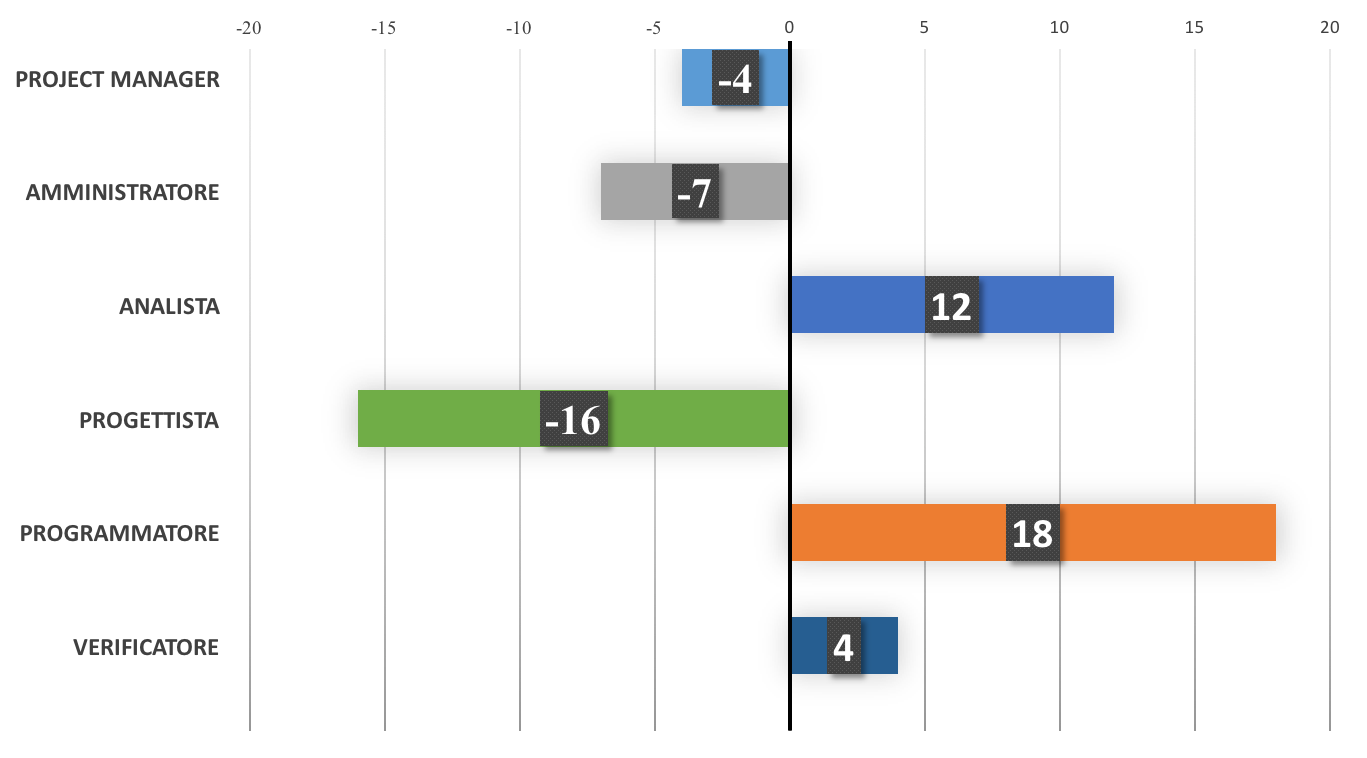
\includegraphics[scale=0.7]{Immagini/GraficiCONS/DIFFORARIA.png}
	\caption{Differenza di ore rendicontate tra quelle preventivate al momento dell'aggiudicazione del capitolato e quelle effettivamente riscontrate a consuntivo}
\end{figure}

Dal consuntivo emerge un aumento di \textbf{18\euro} con un costo totale che ora ammonta a \textbf{13639\euro}, rispetto ai \textbf{13621\euro} preventivati nella pianificazione ed al momento dell'aggiudicazione del capitolato.\\
Il gruppo quindi non è riuscito a rientrare ed a rispettare il preventivo di \textbf{13621\euro} fissato al momento dell'aggiudicazione del capitolato ma si ritiene comunque soddisfatto di essere riuscito a mantenere i costi sulla linea di quelli preventivati all'inizio del progetto, anche in seguito alle diverse problematiche riscontrate.